% 컴파일: XeLaTeX (또는 tectonic)
% 글꼴: 함초롬바탕/함초롬돋움 (한컴오피스 설치 시 Windows 글꼴 폴더의 HANBatang*.ttf, HANDotum*.ttf)
\documentclass[10pt,twocolumn,a4paper]{article}

\usepackage[a4paper,top=22mm,bottom=22mm,left=17mm,right=17mm,columnsep=7mm]{geometry}
\usepackage{kotex}
\setmainhangulfont{HANBatang.ttf}[Path=/mnt/c/Windows/Fonts/,BoldFont=HANBatangB.ttf]
\setsanshangulfont{HANDotum.ttf}[Path=/mnt/c/Windows/Fonts/,BoldFont=HANDotumB.ttf]
\XeTeXlinebreaklocale ""
\xetexkofontregime{latin}

\usepackage{amsmath,amssymb,bm}
\usepackage{graphicx}
\usepackage{booktabs}
\usepackage{caption}
\usepackage{titlesec}
\usepackage[hidelinks]{hyperref}

\graphicspath{{../docs/}}
\captionsetup{font=small,labelfont=bf,labelsep=period}
\captionsetup[table]{position=top}
\titleformat{\section}{\sffamily\bfseries\large\raggedright}{\thesection.}{0.5em}{}
\titleformat{\subsection}{\sffamily\bfseries\normalsize\raggedright}{\thesubsection}{0.5em}{}
\titlespacing*{\section}{0pt}{1.2ex}{0.6ex}
\titlespacing*{\subsection}{0pt}{1ex}{0.4ex}
\renewcommand{\tablename}{Table}
\renewcommand{\figurename}{Fig.}
\renewcommand{\refname}{References}
\linespread{1.1}
\hyphenation{Section}

\begin{document}

\twocolumn[{%
\begin{center}
  {\sffamily\bfseries\LARGE 가상 공정 데이터를 이용한\\[2pt]웨이퍼 양불 판정 모델의 구현과 분석\par}
  \vspace{10pt}
  {\large 정현욱\par}
  \vspace{2pt}
  {\small 고려대학교 세종 지능형반도체공학과\par}
  \vspace{12pt}
\end{center}
\noindent\rule{\textwidth}{0.4pt}
\vspace{2pt}

\noindent{\sffamily\bfseries Abstract}\par
\vspace{2pt}
\noindent\small
반도체 공장에서 양불 판정 모델을 학습시키려면 많은 양의 웨이퍼 데이터가 필요하지만, 실제
데이터는 비용이 크고 다양한 공정 조건에서 고르게 모으기도 어렵다. 본 프로젝트에서는 공정을
모사하는 시뮬레이터(가상 fab)를 만들고, 여기서 생성한 데이터로 EDS 단계의 판정 모델을
학습시켜 보았다. 시뮬레이터와 분류기는 외부 머신러닝 프레임워크 없이 numpy로 직접
구현하였다. 데이터를 만들 때 라벨은 참값으로 정하되 모델에는 노이즈가 섞인 측정값만
보여 주어, 스펙 경계 근처에서는 어떤 모델로도 판정이 완전히 정확할 수 없도록 하였다.
양품 영역이 여러 스펙을 동시에 만족해야 하는 상자 모양이라 단층 퍼셉트론은 불량을 거의
걸러내지 못했고(불량 F1 13.85\%), 은닉층을 둔 MLP는 이 문제를 풀어냈다(78.08\%).
스펙 경계까지의 거리를 특징으로 넣어 주면 퍼셉트론의 성능도 상당 부분 회복되었다.
끝으로 물리 상수를 일부러 다르게 둔 두 번째 시뮬레이터를 현실 fab으로 가정하고 전이
실험을 해 보았는데, 여러 공정 조건을 담은 가상 데이터만으로 학습한 모델이 단일 조건의
현실 fab 데이터 전량으로 학습한 모델보다 나은 결과를 보였다. 다만 이 비교에는 조건 수의
차이가 섞여 있고, 현실 fab 역시 시뮬레이터라는 점에서 해석에 주의가 필요하다.

\vspace{4pt}
\noindent\textbf{Keywords:} 가상 fab, 디지털 트윈, 웨이퍼 양불 판정, 다층 퍼셉트론, 역전파, sim2real
\vspace{4pt}

\noindent\rule{\textwidth}{0.4pt}
\vspace{10pt}
}]

% ------------------------------------------------------------------
\section{Introduction}

머신러닝을 처음 배울 때는 대개 잘 정리된 데이터셋이 주어진다. 하지만 반도체 공장의 사정은
다르다. 데이터 한 줄을 얻으려면 웨이퍼 한 장이 수십 단계의 공정과 측정을 실제로 거쳐야 하고,
수율이 높은 라인일수록 모델이 정작 배워야 할 불량 샘플은 드물다. 공정 조건을 바꿔 가며
데이터를 모으는 일은 더 어렵다. 양산 중인 라인의 설정을 실험 목적으로 바꾸는 것은 같은
조건에서 웨이퍼를 더 흘리는 것과는 비교할 수 없을 만큼 부담이 크다.

이런 제약 때문에 공정 물리를 근사한 시뮬레이터로 가상 웨이퍼를 대량으로 만들고, 그 데이터로
판정 모델을 학습시키는 방법이 관심을 받고 있다. 산업계에서 디지털 트윈이라고 부르는 접근이다.
본 프로젝트는 이 아이디어를 작은 규모로나마 직접 구현해 보면서, 가상 데이터로 양불 판정을
학습할 수 있는지, 문제를 풀려면 어느 정도 복잡한 모델이 필요한지, 그리고 시뮬레이터의 물리가
현실과 어긋나 있을 때에도 가상 데이터가 쓸모 있는지를 차례로 살펴본 기록이다.

분류기는 scikit-learn이나 PyTorch를 쓰지 않고 numpy로 구현하였다. 라이브러리가 대신
해 주던 계산, 특히 역전파를 직접 작성하고 검증해 보는 것이 이 프로젝트의 또 다른 목표였기
때문이다.

본문에서 자주 쓰는 용어를 미리 정리해 둔다. EDS는 완성된 웨이퍼를 전기적으로 측정해 양품과
불량을 가르는 검사 단계로, 본 프로젝트의 모델이 흉내 내려는 대상이다. 스펙은 제품이 만족해야
하는 값의 범위로, 물리 법칙이 아니라 제품 요구사항에 해당한다. run은 시뮬레이터를 한 번
실행한 단위를 가리키며, 한 run에서 나온 웨이퍼 2만 장은 모두 같은 공정 조건을 공유한다.

% ------------------------------------------------------------------
\section{Virtual Fab Design}

\subsection{Process Parameters and Specifications}

시뮬레이터가 만드는 웨이퍼 한 장은 Table~\ref{tab:spec}의 다섯 가지 값으로 표현된다. 다섯 값이
모두 스펙 안에 들어와야 양품이고, 하나라도 벗어나면 불량으로 본다. 기하학적으로 보면 양품
영역은 5차원 공간 속의 상자(box)이며, 뒤에서 다룰 모델 간 성능 차이는 대부분 이 상자 모양에서
비롯된다.

\begin{table}[t]
\centering\small
\caption{공정 파라미터와 스펙 범위}
\label{tab:spec}
\begin{tabular}{lll}
\toprule
파라미터 & 의미 & 스펙 \\
\midrule
Vth [V]      & 문턱전압      & 0.67 -- 0.73 \\
Oxide [nm]   & 게이트 산화막 두께 & 97 -- 103 \\
Leakage [nA] & 누설전류      & $\le 10$ \\
CD [nm]      & 게이트 선폭    & 43.5 -- 46.5 \\
Temp [°C]    & 공정 온도      & 23 -- 27 \\
\bottomrule
\end{tabular}
\end{table}

실제 라인은 시기마다 상태가 조금씩 달라진다. 이를 반영하기 위해 각 파라미터의 중심값과
산포를 run마다 정해진 범위 안에서 새로 뽑도록 하였고, 그 결과 run이 바뀌면 데이터의 분포도
함께 달라진다.

\subsection{Physical Coupling Between Parameters}

다섯 값을 서로 독립적으로 뽑으면 공정 데이터라기보다 난수표에 가깝다. 그래서 소자 물리를
단순화한 관계식을 넣어 값들이 서로 영향을 주도록 하였다. 게이트 산화막이 두꺼워지면
문턱전압은 올라가고 누설전류는 줄어들며, 선폭이 좁아지면 short channel 효과로 문턱전압이
내려가고 누설전류가 늘어난다. 온도가 오르면 누설전류는 지수적으로 커진다. 이 관계들의 세기는
몇 개의 결합 계수로 정해 두었고, Section~\ref{sec:sim2real}에서는 이 계수를 바꾼 두 번째 시뮬레이터를 만들어
사용한다.

\subsection{True-Value Labels and Measured Features}

이 시뮬레이터에서 가장 중요한 설계 결정은 라벨과 특징을 서로 다른 값으로 만든 것이다. 웨이퍼의 참값을
$\bm{x}$, 측정 노이즈를 $\bm{\varepsilon}$이라고 하면 라벨과 특징은 다음과 같다.
\begin{align}
  y &= \mathbf{1}\!\left[\,\bm{x} \in \text{Spec}\,\right], \label{eq:label}\\
  \tilde{\bm{x}} &= \bm{x} + \bm{\varepsilon}. \label{eq:meas}
\end{align}
라벨 $y$는 시뮬레이터만 알고 있는 참값으로 판정하고, 데이터셋에는 측정값 $\tilde{\bm{x}}$만
남긴다. 실제 공장에서도 사람이 볼 수 있는 것은 검사 장비가 보고한 측정값뿐이므로 이 편이 더
현실에 가깝다고 판단하였다.

이렇게 하면 참 Vth가 스펙 상한을 아주 조금 넘은 웨이퍼가 측정 오차 때문에 스펙 안쪽 값으로
기록되는 일이 생긴다. 모델 입장에서는 양품처럼 보이지만 실제 라벨은 불량이다. 스펙 경계 근처에
있는 웨이퍼는 측정값만으로 가려낼 수 없으므로 어떤 모델도 100\%의 정확도에 이를 수 없고,
문제가 지나치게 쉬워지는 것을 막아 준다. 이 성질은 코드에서 라벨을 먼저 판정한 다음 노이즈를
더하는 순서로 지켜지며, 순서를 바꾸면 사라진다.

\subsection{Run-Level Train/Test Split}

학습 데이터와 평가 데이터를 나눌 때는 웨이퍼를 섞지 않고 run을 통째로 떼어 평가에 썼다. 같은
run의 웨이퍼는 공정 조건이 같기 때문에, 웨이퍼 단위로 나누면 평가용 웨이퍼와 같은 조건을 학습
때 이미 본 셈이 되어 성능이 부풀려진다. run 단위로 나누면 학습 때 본 적 없는 공정 조건에서도
판정이 되는지를 확인할 수 있다.

% ------------------------------------------------------------------
\section{Classification Models}

\subsection{Single-Layer Perceptron}

가장 먼저 시도한 모델은 퍼셉트론\cite{rosenblatt}이다. 입력의 가중합
$\bm{w}^\top\tilde{\bm{x}} + b$의 부호로 클래스를 정하는 모델로, 공간을 초평면 하나로 나누는
것과 같다. 데이터가 선형으로 나뉘지 않으면 퍼셉트론의 가중치는 수렴하지 못하고 계속 흔들리기
때문에, 학습 도중 가장 성능이 좋았던 가중치를 따로 보관해 두는 pocket 알고리즘\cite{gallant}을
함께 사용하였다. 입력은 학습 데이터의 평균과 표준편차로 표준화하였다.

\subsection{Structural Limitation of the Perceptron}\label{sec:limit}

Vth 하나만 놓고 보면 문제가 분명해진다. 양품 구간 $[0.67, 0.73]$은 가운데에 있고 불량은
양쪽에 흩어져 있는데, 퍼셉트론이 만들 수 있는 규칙은 어떤 값보다 크면 양품이거나 작으면 양품인
형태뿐이다. 가운데 구간만 양품이라는 규칙은 초평면 하나로는 표현할 수 없다\cite{minsky}.
차원이 다섯으로 늘어나면 불량은 상자의 모든 면 바깥에 놓이게 되어 상황이 더 나빠진다.
실제로 학습 로그를 보면 epoch이 지나도 오분류를 고치는 횟수가 줄지 않았는데, 이는 학습이
부족해서가 아니라 모델 구조 자체의 한계로 보는 것이 맞다.

\subsection{Multilayer Perceptron (MLP)}

이 한계를 넘기 위해 은닉층을 하나 둔 MLP를 구현하였다. 은닉층의 ReLU 뉴런 16개가 각자 하나의
초평면 역할을 하고 출력층이 이를 조합하므로, 여러 초평면으로 둘러싸인 영역을 표현할 수 있다.
출력층에는 sigmoid를 써서 결과를 웨이퍼가 양품일 확률
$p = P(\text{양품}\mid\tilde{\bm{x}})$로 해석할 수 있게 하였다.

역전파\cite{rumelhart}는 직접 작성하였고, 가중치 초기화에는 He 초기화\cite{he}를 사용하였다.
필요하면 L2 정규화를 켤 수 있도록 했지만 기본 설정에서는 쓰지 않았다. 학습은 배치 크기 256의
미니배치 경사하강법으로 진행하였다.

\subsection{Cost Asymmetry and Class Weighting}

공정에서는 두 가지 오류의 무게가 다르다. 불량을 양품으로 잘못 통과시키면 그대로 고객에게
전달되지만, 양품을 불량으로 버리면 웨이퍼 한 장을 잃는 데 그친다. 그런데 데이터의 대부분이
양품이라 아무 조치 없이 학습하면 모델은 양품 쪽으로 기울기 쉽다. 이를 보정하기 위해 불량
샘플의 손실에 가중치 $w_f$를 곱한 교차 엔트로피를 사용하였다.
\begin{equation}
\begin{split}
  \mathcal{L} = -\frac{1}{N}\sum_{i=1}^{N} c_i \big[\, y_i \log p_i
               + (1-y_i)\log(1-p_i) \,\big] \\
               + \frac{\lambda}{2}\sum_{l}\lVert W_l \rVert_F^2
\end{split}
\end{equation}
여기서 $c_i$는 불량($y_i = 0$)일 때 $w_f$, 양품일 때 1이며, 기본값으로 $w_f = 5$,
$\lambda = 0$을 사용하였다.

Table~\ref{tab:weight}에서 보듯 가중치를 주어도 F1은 거의 그대로이고, 대신 precision과 recall의
균형이 recall 쪽으로 옮겨 간다. 이 가중치는 모델을 전반적으로 좋게 만드는 장치라기보다 어떤
오류를 더 피할지를 정하는 장치로 이해하는 것이 맞다.

\begin{table}[t]
\centering\small
\caption{클래스 가중의 효과 (불량 = positive)}
\label{tab:weight}
\begin{tabular}{lcc}
\toprule
 & 가중 없음 & $w_f = 5$ \\
\midrule
Precision & 86.24\% & 70.50\% \\
Recall    & 71.25\% & \textbf{87.47\%} \\
F1        & 78.03\% & 78.08\% \\
\bottomrule
\end{tabular}
\end{table}

\begin{figure*}[t]
\centering
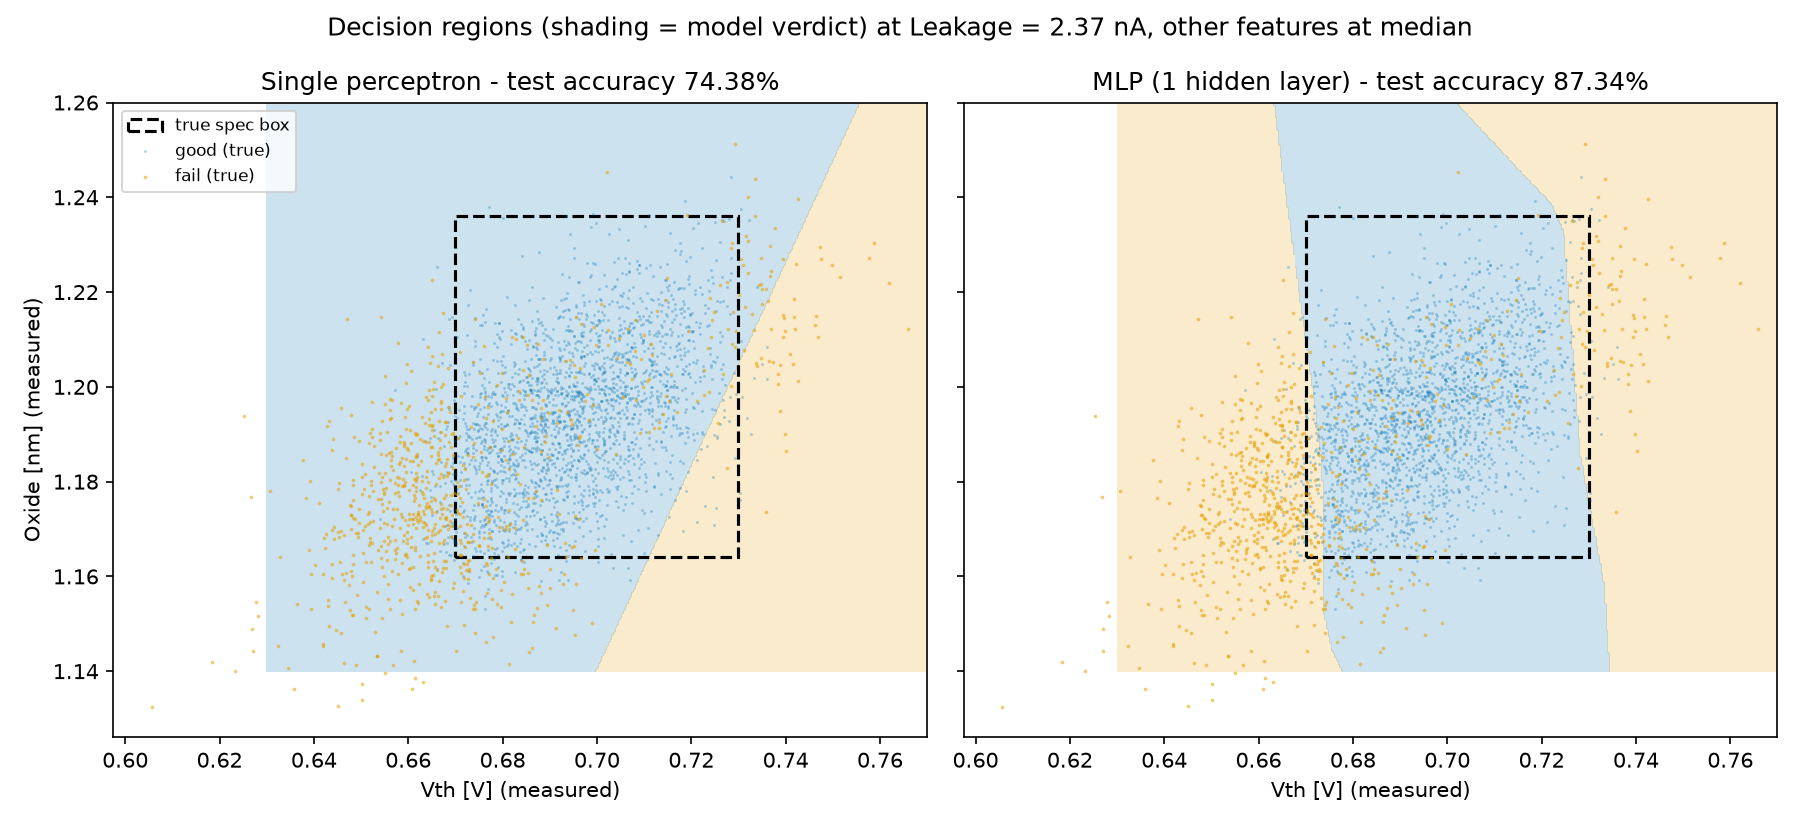
\includegraphics[width=0.92\textwidth]{decision_boundary.png}
\caption{Vth--Oxide 평면에 투영한 결정 경계(나머지 3개 파라미터는 중앙값으로 고정).
점선은 실제 스펙 상자이며, 두 모델은 Table~\ref{tab:main}과 같은 설정으로 학습하였다.}
\label{fig:boundary}
\end{figure*}

% ------------------------------------------------------------------
\section{Experimental Setup}

\subsection{Dataset}

시뮬레이터를 12번 실행해 웨이퍼 24만 장을 만들었고, 이 중 10개 run으로 학습하고 나머지
2개 run으로 평가하였다. run마다 사용한 난수 시드를 기록해 두었기 때문에 같은 데이터를 언제든
다시 만들 수 있다.

\subsection{Evaluation Metrics}

평가 데이터의 약 4분의 3이 양품이어서, 모든 웨이퍼를 양품이라고만 답해도 정확도는 74\%를
넘는다. 정확도만으로는 모델이 무엇을 배웠는지 알기 어렵기 때문에, 불량을 positive로 두고
precision, recall, F1을 주로 보았다. 판정 기준값과 무관한 판별 능력은 ROC AUC와 PR
AP\cite{davis,saito}로 함께 확인하였다.

\subsection{Implementation Verification and Reproducibility}

역전파를 손으로 작성한 만큼 기울기가 맞게 계산되는지부터 확인하였다. 손실을 유한차분으로
미분한 값과 역전파 결과를 비교했으며, 은닉층 수와 정규화 설정을 바꾼 여섯 가지 구성 모두에서
상대오차가 $10^{-6}$ 이하로 나왔다.

본문에 실은 결과는 모두 기본 시드로 얻은 값이다. 시드를 바꿔 10번 학습했을 때 MLP의 F1은
표준편차가 약 1.8\%p였으므로, 1\%p 정도의 차이는 의미 있게 해석하지 않았다.

% ------------------------------------------------------------------
\section{Results}\label{sec:results}

\subsection{Perceptron vs. MLP}

\begin{table}[t]
\centering\small
\caption{퍼셉트론과 MLP의 성능 (불량 = positive)}
\label{tab:main}
\begin{tabular}{lcc}
\toprule
지표 & 퍼셉트론 & MLP (은닉 16) \\
\midrule
정확도    & 74.38\% & 87.34\% \\
Precision & 51.82\% & 70.50\% \\
Recall    & \textbf{8.00\%} & \textbf{87.47\%} \\
F1        & 13.85\% & 78.08\% \\
ROC AUC   & 0.250 & 0.950 \\
PR AP     & 0.238 & 0.890 \\
\bottomrule
\end{tabular}
\end{table}

Table~\ref{tab:main}은 두 모델의 결과를 정리한 것이다. 퍼셉트론은 불량 대부분을 양품으로
통과시켰고, 정확도도 모두 양품이라고 답하는 경우와 사실상 다르지 않았다. Section~\ref{sec:limit}에서 예상한
그대로의 결과이다. 시드를 바꿀 때마다 결과가 크게 달라진 것도 같은 맥락으로 이해할 수 있는데,
수렴하지 못하고 흔들리는 모델에서 pocket 알고리즘이 어느 시점의 가중치를 고르느냐에 따라
경계가 달라지기 때문이다.

퍼셉트론의 ROC AUC는 무작위로 찍는 수준인 0.5보다도 낮았는데, 그 이유는 다음과 같다.
퍼셉트론의 점수는 한 방향으로만 커지는데 불량은 상자 바깥 모든 방향에 있으니, 점수축의 한쪽
끝을 불량으로 보면 반대쪽 끝에 있는 불량은 오히려 가장 양품다운 웨이퍼로 순위가 매겨진다.
불량을 놓치는 데 그치지 않고 순서조차 거꾸로 매기는 셈이다.

Fig.~\ref{fig:boundary}는 두 모델의 결정 경계를 Vth--Oxide 평면에 투영한 것이다. 퍼셉트론은
평면을 대각선으로 한 번 나눌 뿐이라 한쪽 방향의 불량을 모두 양품으로 판정한다. MLP는 Vth
방향으로 스펙의 하한과 상한을 모두 따라가는 영역을 학습했는데, 퍼셉트론이 구조적으로 만들 수
없던 바로 그 규칙이다. Oxide 방향의 경계는 그림 범위 안에서 닫히지 않았다. 학습 데이터에서
Oxide가 스펙을 벗어난 웨이퍼가 Vth에 비해 훨씬 적어, 그 방향의 경계를 배울 근거가 부족했던
것으로 보인다.

\subsection{Decision Threshold and Operating Point}

MLP는 확률을 내놓기 때문에 몇 이상을 양품으로 볼지, 즉 판정 기준값 $t$를 사용하는 쪽에서
정할 수 있다. Table~\ref{tab:cutoff}처럼 $t$를 높이면 불량은 더 많이 잡히지만 그만큼 멀쩡한
웨이퍼도 많이 버려진다. F1만 따지면 0.3 부근이 가장 좋지만, 불량 유출을 무엇보다 피해야 하는
라인이라면 0.9로 높여 불량을 거의 다 잡는 쪽을 택할 수도 있다. 어느 지점이 옳은지는 지표가
아니라 두 오류의 비용을 따져 결정할 문제라고 생각한다. 참고로 $t = 0.9$에서의 recall은
시드를 바꿔도 거의 변하지 않아, 이 운영점에서는 모델이 안정적으로 동작하였다.

\begin{table}[t]
\centering\small
\caption{cutoff에 따른 운영점 (MLP)}
\label{tab:cutoff}
\begin{tabular}{cccc}
\toprule
cutoff & Precision & Recall & F1 \\
\midrule
0.1 & 91.86\% & 60.78\% & 73.16\% \\
0.3 & 79.86\% & 78.38\% & \textbf{79.11\%} \\
0.5 & 70.50\% & 87.47\% & 78.08\% \\
0.7 & 60.29\% & 93.47\% & 73.30\% \\
0.9 & 46.09\% & \textbf{98.23\%} & 62.75\% \\
\bottomrule
\end{tabular}
\end{table}

\subsection{Effect of Derived Margin Features}

퍼셉트론이 실패한 원인이 상자 모양에 있다면, 상자를 모델 대신 특징 쪽에서 풀어 주면 어떨까
하는 생각으로 다음 실험을 하였다. 스펙 한계는 공장이 이미 알고 있는 제품 요구사항이므로 모델에
알려 주어도 정보 누설이 아니다. 그래서 각 측정값이 가장 가까운 스펙 경계에서 얼마나 떨어져
있는지를 특징으로 추가하였다. 양쪽 스펙 $[s_{\min}, s_{\max}]$을 가진 파라미터 $j$에 대해서는
\begin{equation}
  m_j = \frac{\min(\tilde{x}_j - s_{\min},\; s_{\max} - \tilde{x}_j)}{(s_{\max} - s_{\min})/2}
\end{equation}
로 정의하였고, 상한만 있는 Leakage는 $m = (s_{\max} - \tilde{x})/s_{\max}$로 두었다. 값이
양수이면 스펙 안쪽, 음수이면 바깥쪽이다. 여기에 이들의 최솟값 $m_{\min}$을 하나 더 추가하였다.
$m_{\min}$이 0 이상이면 양품이라는 규칙은 한 축 위에서의 선형 분할이므로, 초평면 하나로 풀 수
없던 문제가 초평면 하나로 풀리는 문제로 바뀌게 된다.

\begin{table}[t]
\centering\small
\caption{margin 특징의 효과}
\label{tab:margin}
\begin{tabular}{llcc}
\toprule
모델 & 특징 & Recall & F1 \\
\midrule
퍼셉트론 & 원본 5개 & 8.00\% & 13.85\% \\
퍼셉트론 & + margin 6개 & \textbf{44.57\%} & \textbf{59.05\%} \\
MLP & 원본 5개 & 87.47\% & 78.08\% \\
MLP & + margin 6개 & 91.16\% & 77.54\% \\
\bottomrule
\end{tabular}
\end{table}

\begin{table}[t]
\centering\small
\caption{두 세계의 물리 결합 계수 차이}
\label{tab:worlds}
\begin{tabular}{lccr}
\toprule
결합 & 트윈 & 현실 fab & 차이 \\
\midrule
Oxide $\rightarrow$ Vth   & 0.010 & 0.013 & +30\% \\
CD $\rightarrow$ Vth      & 0.004 & 0.006 & +50\% \\
Oxide $\rightarrow$ Leak  & $-0.30$ & $-0.36$ & +20\% \\
CD $\rightarrow$ Leak     & $-0.05$ & $-0.03$ & $-40\%$ \\
Temp $\rightarrow$ Leak   & 0.03 & 0.05 & +67\% \\
\bottomrule
\end{tabular}
\end{table}

\begin{table}[t]
\centering\small
\caption{현실 fab 데이터 예산에 따른 불량 F1 (\%, 시드 10개 평균 $\pm$ 표준편차)}
\label{tab:sim2real}
\begin{tabular}{rcc}
\toprule
현실 fab 데이터 & scratch & fine-tune \\
\midrule
250장    & $31.67 \pm 2.54$ & $\mathbf{72.83 \pm 0.82}$ \\
1,000장  & $35.22 \pm 2.83$ & $\mathbf{73.49 \pm 0.98}$ \\
4,000장  & $43.21 \pm 3.67$ & $\mathbf{72.90 \pm 0.68}$ \\
16,000장 & $60.20 \pm 3.13$ & $\mathbf{73.46 \pm 0.28}$ \\
\midrule
\multicolumn{3}{l}{zero-shot (0장): 73.62} \\
\multicolumn{3}{l}{oracle (2만 장 전량): $60.78 \pm 4.37$} \\
\bottomrule
\end{tabular}
\end{table}

결과는 Table~\ref{tab:margin}과 같다. 퍼셉트론의 F1은 네 배 넘게 올라 실제로 쓸 만한 수준에
가까워졌다. 학습된 가중치를 살펴보니 퍼셉트론은 다른 어떤 특징보다 $m_{\min}$에 큰 가중치를
두고 있었는데, 규칙의 구조를 특징으로 넣어 주자 모델이 그 축을 스스로 찾아낸 것이다. 그래도
MLP에는 미치지 못했다. $m_{\min}$이 규칙을 완전히 선형으로 바꿔 주는 것은 참값으로 계산할
때의 이야기이고, 실제로는 노이즈가 섞인 측정값으로 계산되기 때문이다.

MLP는 margin 특징을 넣어도 F1이 거의 달라지지 않았다. 은닉층이 이미 상자를 표현할 수 있으니
같은 정보를 한 번 더 받아도 얻을 것이 없었던 셈이다. 두 결과를 함께 보면, 문제를 푸는 데
필요한 표현력은 모델에서 가져올 수도 있고 특징에서 가져올 수도 있으며, 한쪽을 보강하면 다른
쪽에 대한 요구가 줄어든다는 점을 확인할 수 있었다.

% ------------------------------------------------------------------
\section{Extended Experiment: Transfer Across Mismatched Physics}\label{sec:sim2real}

\subsection{Motivation and Setup}

Section~\ref{sec:results}까지의 실험은 학습과 평가가 모두 같은 시뮬레이터 안에서 이루어졌다. 시뮬레이터가 곧
현실인 셈이니 결과가 잘 나오는 것은 어찌 보면 당연하고, 시뮬레이터가 현실과 다를 때에도
쓸모가 있는지는 아직 알 수 없다. 현실을 완벽하게 재현하는 시뮬레이터는 없으므로, 이 질문에
답하지 못하면 앞의 결과도 의미가 줄어든다.

이를 확인하기 위해 현실 fab 역할을 할 두 번째 시뮬레이터를 따로 만들었다. Table~\ref{tab:worlds}에
정리한 것처럼 물리 결합 계수를 원래 시뮬레이터(이하 트윈)와 20--67\% 다르게 두었고, 측정
노이즈도 온도를 제외하면 더 크게 설정하였다. 스펙은 제품 요구사항이므로 두 세계에서 같다.
트윈은 이런 차이를 알지 못하므로, 트윈이 만든 데이터는 잘못된 물리에서 나온, 체계적으로
치우친 데이터가 된다.

비교한 방법은 세 가지이다. 현실 fab 데이터만으로 처음부터 학습하는 방법(scratch), 트윈
데이터로만 학습해 그대로 적용하는 방법(zero-shot), 트윈으로 먼저 학습한 뒤 현실 fab 데이터로
추가 학습하는 방법(fine-tune)이다. 트윈 데이터는 12가지 공정 조건을 담고 있고, 현실 fab에서
쓸 수 있는 데이터는 run 하나, 즉 단일 조건의 2만 장으로 제한하였다. 평가는 현실 fab의 다른
run 두 개에서 하였고, 결과는 시드 10개의 평균과 표준편차로 정리하였다.

\begin{figure}[t]
\centering
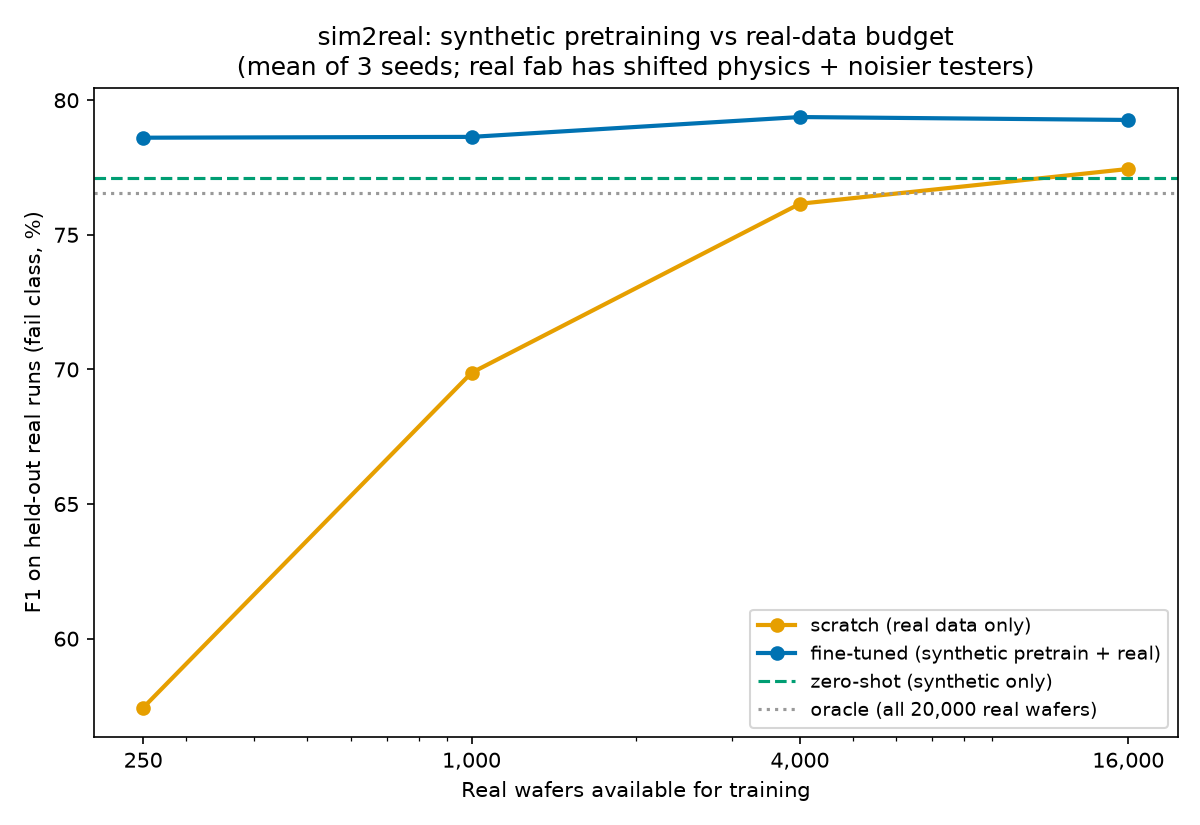
\includegraphics[width=\columnwidth]{sim2real.png}
\caption{현실 fab 데이터 예산에 따른 전략별 불량 F1.}
\label{fig:sim2real}
\end{figure}

\subsection{Results}

결과는 Table~\ref{tab:sim2real}과 Fig.~\ref{fig:sim2real}에 정리하였다. 가장 눈에 띄는 것은 현실
fab 데이터를 한 장도 쓰지 않은 zero-shot 모델이, 현실 fab 데이터 2만 장을 모두 써서 학습한
모델(oracle)보다 F1이 10\%p 넘게 높았다는 점이다. zero-shot은 모델 하나로 얻은 단일 값이지만,
oracle의 표준편차를 두 배로 잡아도 차이는 남는다.

현실 fab 데이터를 늘려 가며 fine-tune한 결과를 보면 그 이유를 짐작할 수 있다. 데이터를
250장에서 16,000장까지 늘려도 fine-tune의 성능은 거의 그대로였다. 현실 fab 데이터가 모두 같은
공정 조건에서 나왔기 때문에, 양을 늘려도 모델이 새로 배울 것이 많지 않았던 것으로 보인다.
반면 트윈 데이터는 여러 조건을 고루 담고 있다. 이렇게 보면 차이를 만든 것은 데이터의 양보다
공정 조건의 다양성에 가깝다. fine-tune이 zero-shot보다 나아지지 않은 것도,
추가 학습에 쓴 데이터 역시 단일 조건이었기 때문으로 보인다.

\subsection{Caveats in Interpretation}

이 결과를 가상 데이터가 실제 데이터보다 낫다는 뜻으로 받아들여서는 곤란하다. zero-shot과
oracle의 비교는 가상과 현실의 비교이면서 동시에 조건 12개와 1개의 비교이기도 하고, 이번
실험만으로는 두 요인을 떼어 놓을 수 없다. 또 두 세계의 차이는 계수의 크기만 다르고 식의
형태는 같은, 파라미터 수준의 불일치였다. 이번 실험으로 말할 수 있는 것은 이 정도의
불일치가 조건 다양성에서 오는 이득을 넘어서지 않았다는 데까지이다. 시뮬레이션의 다양성을
넓혀 현실로의 전이를 노리는 domain randomization\cite{tobin}의 관점과도 맞닿아 있는
결과라고 생각한다.

% ------------------------------------------------------------------
\section{Limitations and Future Work}

가장 큰 한계는 Section~\ref{sec:sim2real}의 현실 fab 역시 시뮬레이터라는 점이다. 물리 상수만 바꾼 또 하나의 가상
세계로 옮겨 간 것이므로 엄밀하게는 sim-to-sim 실험이며, 실제 공정 데이터로는 검증하지
못하였다. 실제 시뮬레이터와 현실 사이의 차이는 계수가 조금 다른 정도가 아니라 변수가 아예
빠져 있거나 시간에 따라 서서히 변하는 등 더 구조적인 형태일 수 있다.

현실 fab 데이터가 단일 조건으로 제한된 것도 결과 해석에 영향을 준다. Section~\ref{sec:sim2real}의 결론 중 상당 부분이 이 제약에서 비롯되기 때문이다. 추가 학습은 한 조건으로
하고 평가는 본 적 없는 다른 조건으로 했기 때문에, 같은 라인의 데이터로 적응시켜 같은 라인에
투입하는 실제 상황과는 거리가 있다. 불일치의 크기도 한 가지로만 시험해서, 차이를 얼마나
키우면 결과가 뒤집히는지는 알지 못한다.

앞으로는 공개된 웨이퍼 데이터처럼 실측 데이터로 검증해 보고, 여러 조건을 담은 현실 fab
데이터에서 fine-tune의 효과를 다시 확인해 보고자 한다. 불일치를 단계적으로 키워 가는 실험이나,
소량의 실데이터로 모델 대신 시뮬레이터의 물리 상수를 맞추는 캘리브레이션과의 비교도 흥미로운
주제가 될 것이다.

% ------------------------------------------------------------------
\section{Conclusion}

본 프로젝트에서는 반도체 공정을 단순화한 가상 fab과 양불 판정 분류기를 numpy만으로 구현하였다.
라벨은 참값으로, 특징은 측정값으로 만들어 판정에 본질적인 불확실성이 남도록 했고, run 단위로
데이터를 나누어 처음 보는 공정 조건에 대한 일반화 성능을 살펴보았다.

양품 영역이 상자 모양이라는 점 때문에 단층 퍼셉트론은 이 문제를 풀 수 없었고, 은닉층을 둔
MLP는 이를 해결하였다. 스펙 경계까지의 거리를 특징으로 주었을 때 퍼셉트론이 상당 부분
회복되는 것을 보면서, 모델의 복잡도와 특징 설계가 서로를 대신할 수 있다는 점도 확인하였다.
물리가 다른 세계로의 전이 실험에서는 여러 조건을 담은 가상 데이터만으로 학습한 모델이 단일
조건의 현실 fab 데이터로 학습한 모델보다 나은 성능을 보였는데, 그 차이는 데이터의 양보다 조건의
다양성과 더 관련이 있어 보인다.

직접 구현한 역전파는 수치 미분으로 검증하였고, 모든 데이터와 결과는 시드로 다시 만들 수 있도록
하였다. 전체 코드와 실행 방법은 프로젝트 저장소의 README에 정리해 두었다.

% ------------------------------------------------------------------
\begin{thebibliography}{9}
\footnotesize
\bibitem{rosenblatt}
F.~Rosenblatt, ``The perceptron: A probabilistic model for information storage and
organization in the brain,'' \emph{Psychological Review}, vol.~65, no.~6, pp.~386--408, 1958.

\bibitem{minsky}
M.~Minsky and S.~Papert, \emph{Perceptrons: An Introduction to Computational Geometry}.
MIT Press, 1969.

\bibitem{gallant}
S.~I.~Gallant, ``Perceptron-based learning algorithms,'' \emph{IEEE Transactions on Neural
Networks}, vol.~1, no.~2, pp.~179--191, 1990.

\bibitem{rumelhart}
D.~E.~Rumelhart, G.~E.~Hinton, and R.~J.~Williams, ``Learning representations by
back-propagating errors,'' \emph{Nature}, vol.~323, pp.~533--536, 1986.

\bibitem{he}
K.~He, X.~Zhang, S.~Ren, and J.~Sun, ``Delving deep into rectifiers: Surpassing human-level
performance on ImageNet classification,'' in \emph{Proc. IEEE International Conference on
Computer Vision (ICCV)}, pp.~1026--1034, 2015.

\bibitem{davis}
J.~Davis and M.~Goadrich, ``The relationship between precision-recall and ROC curves,'' in
\emph{Proc. International Conference on Machine Learning (ICML)}, pp.~233--240, 2006.

\bibitem{saito}
T.~Saito and M.~Rehmsmeier, ``The precision-recall plot is more informative than the ROC plot
when evaluating binary classifiers on imbalanced datasets,'' \emph{PLoS ONE}, vol.~10, no.~3,
e0118432, 2015.

\bibitem{tobin}
J.~Tobin, R.~Fong, A.~Ray, J.~Schneider, W.~Zaremba, and P.~Abbeel, ``Domain randomization for
transferring deep neural networks from simulation to the real world,'' in \emph{Proc. IEEE/RSJ
International Conference on Intelligent Robots and Systems (IROS)}, pp.~23--30, 2017.
\end{thebibliography}

\end{document}
